% This file was created with tikzplotlib v0.10.1.post9.
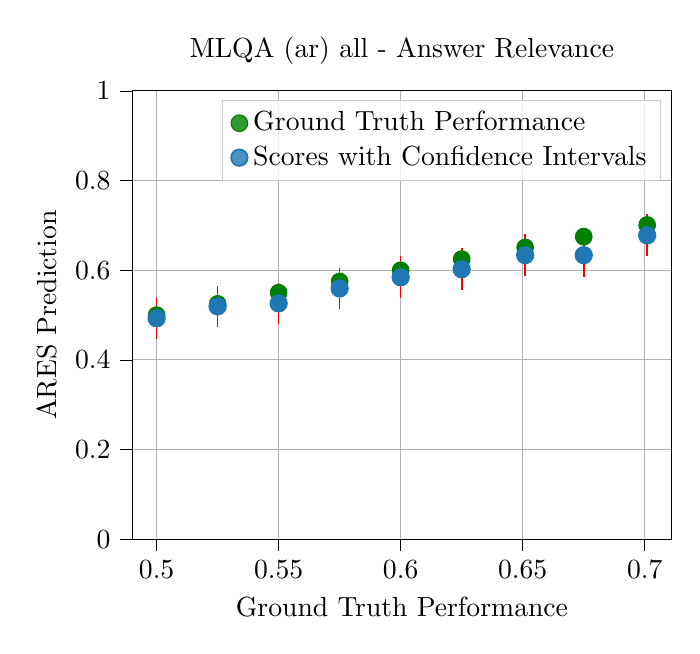
\begin{tikzpicture}

\definecolor{darkgrey176}{RGB}{176,176,176}
\definecolor{green01270}{RGB}{0,127,0}
\definecolor{lightgrey204}{RGB}{204,204,204}
\definecolor{steelblue31119180}{RGB}{31,119,180}

\begin{axis}[
legend cell align={left},
legend style={
  fill opacity=0.8,
  draw opacity=1,
  text opacity=1,
  draw=lightgrey204,
  mark options={mark size=3}
},
tick align=outside,
tick pos=left,
title={MLQA (ar) all - Answer Relevance},
x grid style={darkgrey176},
xlabel={Ground Truth Performance},
xmajorgrids,
xmin=0.48995, xmax=0.71105,
xtick style={color=black},
y grid style={darkgrey176},
ylabel={ARES Prediction},
ymajorgrids,
ymin=0, ymax=1,
ytick style={color=black}
]
\addplot [draw=green01270, fill=green01270, mark size=3pt, mark=*, only marks]
table{%
x  y
0.5 0.5
0.525 0.525
0.55 0.55
0.575 0.575
0.6 0.6
0.625 0.625
0.651 0.651
0.675 0.675
0.701 0.701
};
\addlegendentry{Ground Truth Performance}
\path [draw=red, semithick]
(axis cs:0.5,0.447)
--(axis cs:0.5,0.538);

\path [draw=red, semithick]
(axis cs:0.525,0.474)
--(axis cs:0.525,0.565);

\path [draw=red, semithick]
(axis cs:0.55,0.48)
--(axis cs:0.55,0.572);

\path [draw=red, semithick]
(axis cs:0.575,0.513)
--(axis cs:0.575,0.606);

\path [draw=red, semithick]
(axis cs:0.6,0.538)
--(axis cs:0.6,0.631);

\path [draw=red, semithick]
(axis cs:0.625,0.555)
--(axis cs:0.625,0.649);

\path [draw=red, semithick]
(axis cs:0.651,0.587)
--(axis cs:0.651,0.681);

\path [draw=red, semithick]
(axis cs:0.675,0.586)
--(axis cs:0.675,0.681);

\path [draw=red, semithick]
(axis cs:0.701,0.631)
--(axis cs:0.701,0.725);

\addplot [semithick, steelblue31119180, mark=*, mark size=3, mark options={solid}, only marks]
table {%
0.5 0.492849099099099
0.525 0.519461697722567
0.55 0.526146220570012
0.575 0.559475218658892
0.6 0.584313725490196
0.625 0.602358324533615
0.651 0.633699633699634
0.675 0.633713416951729
0.701 0.677909270216963
};
\addlegendentry{Scores with Confidence Intervals}
\end{axis}

\end{tikzpicture}
